% Options for packages loaded elsewhere
\PassOptionsToPackage{unicode}{hyperref}
\PassOptionsToPackage{hyphens}{url}
%
\documentclass[
]{article}
\usepackage{amsmath,amssymb}
\usepackage{lmodern}
\usepackage{iftex}
\ifPDFTeX
  \usepackage[T1]{fontenc}
  \usepackage[utf8]{inputenc}
  \usepackage{textcomp} % provide euro and other symbols
\else % if luatex or xetex
  \usepackage{unicode-math}
  \defaultfontfeatures{Scale=MatchLowercase}
  \defaultfontfeatures[\rmfamily]{Ligatures=TeX,Scale=1}
\fi
% Use upquote if available, for straight quotes in verbatim environments
\IfFileExists{upquote.sty}{\usepackage{upquote}}{}
\IfFileExists{microtype.sty}{% use microtype if available
  \usepackage[]{microtype}
  \UseMicrotypeSet[protrusion]{basicmath} % disable protrusion for tt fonts
}{}
\makeatletter
\@ifundefined{KOMAClassName}{% if non-KOMA class
  \IfFileExists{parskip.sty}{%
    \usepackage{parskip}
  }{% else
    \setlength{\parindent}{0pt}
    \setlength{\parskip}{6pt plus 2pt minus 1pt}}
}{% if KOMA class
  \KOMAoptions{parskip=half}}
\makeatother
\usepackage{xcolor}
\IfFileExists{xurl.sty}{\usepackage{xurl}}{} % add URL line breaks if available
\IfFileExists{bookmark.sty}{\usepackage{bookmark}}{\usepackage{hyperref}}
\hypersetup{
  pdftitle={Script Package},
  hidelinks,
  pdfcreator={LaTeX via pandoc}}
\urlstyle{same} % disable monospaced font for URLs
\usepackage[margin=1in]{geometry}
\usepackage{color}
\usepackage{fancyvrb}
\newcommand{\VerbBar}{|}
\newcommand{\VERB}{\Verb[commandchars=\\\{\}]}
\DefineVerbatimEnvironment{Highlighting}{Verbatim}{commandchars=\\\{\}}
% Add ',fontsize=\small' for more characters per line
\usepackage{framed}
\definecolor{shadecolor}{RGB}{248,248,248}
\newenvironment{Shaded}{\begin{snugshade}}{\end{snugshade}}
\newcommand{\AlertTok}[1]{\textcolor[rgb]{0.94,0.16,0.16}{#1}}
\newcommand{\AnnotationTok}[1]{\textcolor[rgb]{0.56,0.35,0.01}{\textbf{\textit{#1}}}}
\newcommand{\AttributeTok}[1]{\textcolor[rgb]{0.77,0.63,0.00}{#1}}
\newcommand{\BaseNTok}[1]{\textcolor[rgb]{0.00,0.00,0.81}{#1}}
\newcommand{\BuiltInTok}[1]{#1}
\newcommand{\CharTok}[1]{\textcolor[rgb]{0.31,0.60,0.02}{#1}}
\newcommand{\CommentTok}[1]{\textcolor[rgb]{0.56,0.35,0.01}{\textit{#1}}}
\newcommand{\CommentVarTok}[1]{\textcolor[rgb]{0.56,0.35,0.01}{\textbf{\textit{#1}}}}
\newcommand{\ConstantTok}[1]{\textcolor[rgb]{0.00,0.00,0.00}{#1}}
\newcommand{\ControlFlowTok}[1]{\textcolor[rgb]{0.13,0.29,0.53}{\textbf{#1}}}
\newcommand{\DataTypeTok}[1]{\textcolor[rgb]{0.13,0.29,0.53}{#1}}
\newcommand{\DecValTok}[1]{\textcolor[rgb]{0.00,0.00,0.81}{#1}}
\newcommand{\DocumentationTok}[1]{\textcolor[rgb]{0.56,0.35,0.01}{\textbf{\textit{#1}}}}
\newcommand{\ErrorTok}[1]{\textcolor[rgb]{0.64,0.00,0.00}{\textbf{#1}}}
\newcommand{\ExtensionTok}[1]{#1}
\newcommand{\FloatTok}[1]{\textcolor[rgb]{0.00,0.00,0.81}{#1}}
\newcommand{\FunctionTok}[1]{\textcolor[rgb]{0.00,0.00,0.00}{#1}}
\newcommand{\ImportTok}[1]{#1}
\newcommand{\InformationTok}[1]{\textcolor[rgb]{0.56,0.35,0.01}{\textbf{\textit{#1}}}}
\newcommand{\KeywordTok}[1]{\textcolor[rgb]{0.13,0.29,0.53}{\textbf{#1}}}
\newcommand{\NormalTok}[1]{#1}
\newcommand{\OperatorTok}[1]{\textcolor[rgb]{0.81,0.36,0.00}{\textbf{#1}}}
\newcommand{\OtherTok}[1]{\textcolor[rgb]{0.56,0.35,0.01}{#1}}
\newcommand{\PreprocessorTok}[1]{\textcolor[rgb]{0.56,0.35,0.01}{\textit{#1}}}
\newcommand{\RegionMarkerTok}[1]{#1}
\newcommand{\SpecialCharTok}[1]{\textcolor[rgb]{0.00,0.00,0.00}{#1}}
\newcommand{\SpecialStringTok}[1]{\textcolor[rgb]{0.31,0.60,0.02}{#1}}
\newcommand{\StringTok}[1]{\textcolor[rgb]{0.31,0.60,0.02}{#1}}
\newcommand{\VariableTok}[1]{\textcolor[rgb]{0.00,0.00,0.00}{#1}}
\newcommand{\VerbatimStringTok}[1]{\textcolor[rgb]{0.31,0.60,0.02}{#1}}
\newcommand{\WarningTok}[1]{\textcolor[rgb]{0.56,0.35,0.01}{\textbf{\textit{#1}}}}
\usepackage{graphicx}
\makeatletter
\def\maxwidth{\ifdim\Gin@nat@width>\linewidth\linewidth\else\Gin@nat@width\fi}
\def\maxheight{\ifdim\Gin@nat@height>\textheight\textheight\else\Gin@nat@height\fi}
\makeatother
% Scale images if necessary, so that they will not overflow the page
% margins by default, and it is still possible to overwrite the defaults
% using explicit options in \includegraphics[width, height, ...]{}
\setkeys{Gin}{width=\maxwidth,height=\maxheight,keepaspectratio}
% Set default figure placement to htbp
\makeatletter
\def\fps@figure{htbp}
\makeatother
\setlength{\emergencystretch}{3em} % prevent overfull lines
\providecommand{\tightlist}{%
  \setlength{\itemsep}{0pt}\setlength{\parskip}{0pt}}
\setcounter{secnumdepth}{-\maxdimen} % remove section numbering
\ifLuaTeX
  \usepackage{selnolig}  % disable illegal ligatures
\fi

\title{Script Package}
\author{}
\date{\vspace{-2.5em}}

\begin{document}
\maketitle

\hypertarget{using-magmaclustr}{%
\section{Using MagmaClustR}\label{using-magmaclustr}}

The \emph{MagmaClustR} package provides functions to 2 différents
algorithms based on Gaussian processes (GPs), \textbf{MAGMA} and
\textbf{MAGMACLUST}.

\textbf{MAGMA} (standing for Multi tAsk Gaussian processes with common
MeAn) propose a multi-task Gaussian process framework to simultaneously
model batches of individuals with a common mean function and a specific
covariance structure. This common mean is defined as a Gaussian process
for which the hyper-posterior distribution is tractable. Therefore an EM
algorithm can be derived for simultaneous hyper-parameters optimisation
and hyper-posterior computation.

While \textbf{MAGMACLUST} is introduced to simultaneously handle
multi-task learning, clustering, and prediction for multiple functional
data. This procedure acts as a model-based clustering method for
functional data as well as a learning step for subsequent predictions
for new tasks. The model is instantiated as a mixture of multi-task GPs
with common mean processes. A variational EM algorithm is derived for
dealing with the optimisation of the hyper-parameters along with the
hyper-posteriors' estimation of latent variables and processes

\textbf{MAGMA} is a model where the specific covariance structure of
each individual is defined through a kernel and its associated set of
hyper-parameters. So to speed-up computations of the stationary kernel,
some of the computational parts of the package are implemented in C++
through the use of the Rcpp package.

\hypertarget{magma}{%
\subsection{MAGMA}\label{magma}}

The magma part of the package use a lot of function to make its
prediction. They can be classified as follows :

\begin{itemize}
\tightlist
\item
  The kernels
\item
  The modification of the kernel to create matrix (or kernel-to-matrices
  in the package)
\item
  The likelihoods
\item
  The gradients
\item
  The EM algorithm
\item
  The training of the data
\item
  The prediction of future timestamps thank to the training of our data
\item
  The plot functions, to have graphic
\end{itemize}

\hypertarget{data-structure}{%
\subsubsection{1. Data structure}\label{data-structure}}

The structure of the data is a tibble or a data frame. There are 3
Required columns that must be identifiable by their names as \emph{ID},
\emph{Input} and \emph{Output}. Additional columns for covariates can be
specified.

The \emph{ID} column contains the unique names/codes used to identify
each individual/task (or batch of data).

The \emph{Input} column should define the variable that is used as
reference for the observations (e.g.~time for longitudinal data).

The \emph{Output} column specifies the observed values (the response
variable).

The data frame can also provide as many covariates as desired, with no
constraints on the column names. These covariates are additional inputs
(explanatory variables) of the models that are also observed at each
reference \emph{Input}.

In case of a simulation, the function \emph{simu\_db} can be use, the
number of individual and observations per individual can be change as
will. It will create by default a batch of data with 10 individuals and
10 observations by individuals.

\begin{Shaded}
\begin{Highlighting}[]
\FunctionTok{simu\_db}\NormalTok{()}
\end{Highlighting}
\end{Shaded}

\begin{verbatim}
## # A tibble: 100 x 4
##    ID    Output Input Covariate
##    <chr>  <dbl> <dbl>     <dbl>
##  1 1       7.98  0.4      -2.79
##  2 1       9.99  1.05      0.43
##  3 1      13.9   1.2       4.53
##  4 1      11.7   2.9       3.38
##  5 1      12.3   3.1       1.82
##  6 1       5.61  3.15     -4.32
##  7 1      11.3   3.9       0.99
##  8 1       3.44  5.25     -4.95
##  9 1      11.3   5.7       3.85
## 10 1      18.2   9.9       1.27
## # ... with 90 more rows
\end{verbatim}

\hypertarget{the-hyper-parameters-and-kernels-structure}{%
\subsubsection{2. The Hyper-parameters and kernels
Structure}\label{the-hyper-parameters-and-kernels-structure}}

The hyper-parameters chosen have to be adapted to the kernels chosen.
Any kernels function can be created but 4 are available by default, and
can be called by a character string.

\begin{itemize}
\tightlist
\item
  ``SE'': the Squared Exponential kernel,
\item
  ``LIN'': the Linear kernel,
\item
  ``PERIO'': the Periodic kernel,
\item
  ``RQ'': the Rational Quadratic kernel.
\end{itemize}

Compound kernels can be created as sums or products of the above
kernels. For combining kernels, simply provide a formula as a character
string where elements are separated by whitespaces (e.g.~``SE +
PERIO''). As the elements are treated sequentially from the left to the
right, the product operator shall always be used before the sum
operators (e.g.~`SE * LIN + RQ' is valid whereas `RQ + SE * LIN' is
not).

The EM algorithm use the partial derivative of the kernel by each
hyper-parameters. If not provide, they can be compute, but this will
take more time and is less precise.

If the kernels chosen is not one of the 4 above, it is recommended to
add a parameters \emph{deriv} of your function kernel which can be NULL
or hyper-parameter's name for the derivative of this hyper-parameter.

In case of a simulation, like the database, a function can be use to
simulate the hyper-parameters. By default, the hyper-parameters are
chosen for the Squared Exponential kernel but you can chose any of the 4
predefined or your own.

\begin{Shaded}
\begin{Highlighting}[]
\FunctionTok{hp}\NormalTok{()}
\end{Highlighting}
\end{Shaded}

\begin{verbatim}
## # A tibble: 1 x 2
##   se_variance se_lengthscale
##         <dbl>          <dbl>
## 1        2.84           2.39
\end{verbatim}

\begin{Shaded}
\begin{Highlighting}[]
\FunctionTok{hp}\NormalTok{(}\StringTok{"PERIO"}\NormalTok{)}
\end{Highlighting}
\end{Shaded}

\begin{verbatim}
## # A tibble: 1 x 3
##   perio_variance perio_lengthscale period
##            <dbl>             <dbl>  <dbl>
## 1           2.63              1.94   1.43
\end{verbatim}

\hypertarget{training-magma-with-an-em-algorithm}{%
\subsubsection{3. Training Magma with an EM
algorithm}\label{training-magma-with-an-em-algorithm}}

The hyper-parameters and the hyper-posterior distribution involved in
Magma can be learned thanks to an EM algorithm implemented in the
function \emph{train\_magma}. By providing a dataset, the model
hypotheses (hyper-prior mean parameter and covariance kernels) and
initialisation values for the hyper-parameters, the function computes
maximum likelihood estimates of the HPs as well as the mean and
covariance parameters of the Gaussian hyper-posterior distribution of
the mean process.

\begin{Shaded}
\begin{Highlighting}[]
\NormalTok{db }\OtherTok{=} \FunctionTok{simu\_db}\NormalTok{()}
\FunctionTok{train\_magma}\NormalTok{(db)}
\end{Highlighting}
\end{Shaded}

\begin{verbatim}
## The 'prior_mean' argument has not been specified. The hyper_prior mean function is thus set to be 0 everywhere.
##  
## The 'ini_hp_0' argument has not been specified. Random values of hyper-parameters for the mean process are used as initialisation.
##  
## The 'ini_hp_i' argument has not been specified. Random values of hyper-parameters for the individal processes are used as initialisation.
##  
## EM algorithm, step 1: 8.83 seconds 
##  
## Value of the likelihood: -295.516180514784 --- Convergence ratio = Inf
##  
## EM algorithm, step 2: 6.52 seconds 
##  
## Value of the likelihood: -284.473996766035 --- Convergence ratio = 0.0388161444430033
##  
## EM algorithm, step 3: 6.01 seconds 
##  
## Value of the likelihood: -284.445211885134 --- Convergence ratio = 0.000101196573884465
##  
## The EM algorithm successfully converged, training is completed. 
## 
\end{verbatim}

\begin{verbatim}
## $hp_0
## # A tibble: 1 x 2
##   se_variance se_lengthscale
##         <dbl>          <dbl>
## 1        3.25          0.840
## 
## $hp_i
## # A tibble: 10 x 4
##    ID    se_variance se_lengthscale noise
##    <chr>       <dbl>          <dbl> <dbl>
##  1 1            3.45           1.73 -2.34
##  2 2            3.45           1.73 -2.34
##  3 3            3.45           1.73 -2.34
##  4 4            3.45           1.73 -2.34
##  5 5            3.45           1.73 -2.34
##  6 6            3.45           1.73 -2.34
##  7 7            3.45           1.73 -2.34
##  8 8            3.45           1.73 -2.34
##  9 9            3.45           1.73 -2.34
## 10 10           3.45           1.73 -2.34
## 
## $post_mean
## # A tibble: 10 x 3
##    Input   Output   Var
##    <dbl>    <dbl> <dbl>
##  1  1.9   6.99     1.76
##  2  2.85  9.48     1.58
##  3  3.15  9.19     1.56
##  4  3.45  8.56     1.56
##  5  4.95  6.36     1.56
##  6  5.5   6.21     1.59
##  7  7.3   0.00355  1.71
##  8  7.6  -1.08     1.70
##  9  7.65 -1.26     1.70
## 10  9.2  -2.28     2.03
## 
## $post_cov
##              1.9       2.85       3.15       3.45      4.95       5.5
## 1.9  1.761342577 1.30286076 1.19728667 1.11528815 0.6180455 0.3792837
## 2.85 1.302860764 1.57824274 1.53163771 1.45369002 0.8809060 0.6980549
## 3.15 1.197286674 1.53163771 1.55889772 1.52241233 1.0012317 0.7970821
## 3.45 1.115288153 1.45369002 1.52241233 1.56057083 1.1353565 0.8949294
## 4.95 0.618045460 0.88090599 1.00123169 1.13535649 1.5623310 1.4339076
## 5.5  0.379283674 0.69805488 0.79708209 0.89492941 1.4339076 1.5902784
## 7.3  0.075672612 0.22763291 0.29558856 0.37282825 0.8436426 1.0922948
## 7.6  0.062731893 0.18258430 0.23911569 0.30624106 0.7312640 0.9362193
## 7.65 0.061412640 0.17587394 0.23021953 0.29538714 0.7119843 0.9062436
## 9.2  0.003334861 0.03326358 0.03844881 0.04695023 0.2068698 0.3595706
##             7.3        7.6       7.65         9.2
## 1.9  0.07567261 0.06273189 0.06141264 0.003334861
## 2.85 0.22763291 0.18258430 0.17587394 0.033263576
## 3.15 0.29558856 0.23911569 0.23021953 0.038448809
## 3.45 0.37282825 0.30624106 0.29538714 0.046950232
## 4.95 0.84364258 0.73126402 0.71198428 0.206869759
## 5.5  1.09229475 0.93621927 0.90624362 0.359570629
## 7.3  1.70535655 1.65700038 1.63671507 0.941729926
## 7.6  1.65700038 1.69913207 1.68763915 1.071366210
## 7.65 1.63671507 1.68763915 1.69808768 1.098173542
## 9.2  0.94172993 1.07136621 1.09817354 2.032482030
## 
## $pred_post
## # A tibble: 10 x 3
##    Input     Mean   Var
##    <dbl>    <dbl> <dbl>
##  1  1.9   6.99     1.76
##  2  2.85  9.48     1.58
##  3  3.15  9.19     1.56
##  4  3.45  8.56     1.56
##  5  4.95  6.36     1.56
##  6  5.5   6.21     1.59
##  7  7.3   0.00355  1.71
##  8  7.6  -1.08     1.70
##  9  7.65 -1.26     1.70
## 10  9.2  -2.28     2.03
## 
## $converged
## [1] TRUE
## 
## $fct_args
## $fct_args$data
## # A tibble: 100 x 4
##    ID    Output Input Covariate
##    <chr>  <dbl> <dbl>     <dbl>
##  1 1     16.5    1.9       4.59
##  2 1     16.6    2.85     -2.02
##  3 1     21.3    3.15      2.89
##  4 1     15.8    3.45     -1.17
##  5 1      8.95   4.95     -2.27
##  6 1     11.3    5.5      -0.08
##  7 1      1.28   7.3      -2.27
##  8 1      0.195  7.6      -1.65
##  9 1     -2.37   7.65     -4.1 
## 10 1      5.47   9.2       3.2 
## # ... with 90 more rows
## 
## $fct_args$prior_mean
## NULL
## 
## $fct_args$ini_hp_0
## # A tibble: 1 x 2
##   se_variance se_lengthscale
##         <dbl>          <dbl>
## 1        3.25          0.840
## 
## $fct_args$ini_hp_i
## # A tibble: 10 x 4
##    ID    se_variance se_lengthscale noise
##    <chr>       <dbl>          <dbl> <dbl>
##  1 1            3.45           1.73 -2.34
##  2 2            3.45           1.73 -2.34
##  3 3            3.45           1.73 -2.34
##  4 4            3.45           1.73 -2.34
##  5 5            3.45           1.73 -2.34
##  6 6            3.45           1.73 -2.34
##  7 7            3.45           1.73 -2.34
##  8 8            3.45           1.73 -2.34
##  9 9            3.45           1.73 -2.34
## 10 10           3.45           1.73 -2.34
## 
## $fct_args$kern_0
## [1] "SE"
## 
## $fct_args$kern_i
## [1] "SE"
## 
## $fct_args$common_hp
## [1] TRUE
## 
## $fct_args$grid_inputs
## NULL
## 
## $fct_args$pen_diag
## [1] 0.01
## 
## $fct_args$n_iter_max
## [1] 25
## 
## $fct_args$cv_threshold
## [1] 0.001
## 
## 
## $training_time
## Time difference of 21.37542 secs
\end{verbatim}

As we can see above, just the database is sufficient to train your
model. However, you can change all the parameters. In particular you can
chose the initial value of the mean process' kernel and of the
individual processes' kernel. Furthermore, the kernel of the mean
process and of the individuals are set to the Squared Exponential
Kernel, but can be change as please.

Learning hyper-parameters of any new individual/task in \textbf{MAGMA}
is required in the prediction procedure. This function \emph{train\_gp}
can be used to learn the hyper-parameters of a simple GP (just ignore
the \emph{post\_cov} argument and consider the \emph{post\_mean}
argument as the GP's mean parameter). When using within \textbf{MAGMA},
by providing data for the new individual/task, the trained model
(hyper-posterior mean and covariance parameters) and initialisation
values for the hyper-parameters, the function computes maximum
likelihood estimates of the hyper-parameters. As above for
\emph{train\_magma}, the function \emph{train\_gp} can be use with only
your database as input but you can change the initial value of your
hyper-parameters.

\begin{Shaded}
\begin{Highlighting}[]
\NormalTok{db }\OtherTok{=} \FunctionTok{simu\_db}\NormalTok{(}\AttributeTok{M =} \DecValTok{1}\NormalTok{, }\AttributeTok{N =} \DecValTok{10}\NormalTok{)}
\FunctionTok{train\_gp}\NormalTok{(db)}
\end{Highlighting}
\end{Shaded}

\begin{verbatim}
## The 'ini_hp' argument has not been specified. Random values of hyper-parameters are used as initialisation.
##  
## The 'post_mean' argument has not been specified. The hyper-posterior mean function is thus set to be 0 everywhere.
## 
\end{verbatim}

\begin{verbatim}
## # A tibble: 1 x 3
##   se_variance se_lengthscale noise
##         <dbl>          <dbl> <dbl>
## 1        5.78           2.34 -16.8
\end{verbatim}

\begin{Shaded}
\begin{Highlighting}[]
\NormalTok{ini\_hp }\OtherTok{=} \FunctionTok{hp}\NormalTok{(}\StringTok{\textquotesingle{}SE\textquotesingle{}}\NormalTok{)}
\NormalTok{post\_mean }\OtherTok{=}\NormalTok{ tibble}\SpecialCharTok{::}\FunctionTok{tibble}\NormalTok{(}\StringTok{\textquotesingle{}Input\textquotesingle{}} \OtherTok{=}\NormalTok{ db}\SpecialCharTok{$}\NormalTok{Input, }\StringTok{\textquotesingle{}Output\textquotesingle{}} \OtherTok{=} \DecValTok{1}\SpecialCharTok{:}\DecValTok{10}\NormalTok{)}
\NormalTok{post\_cov }\OtherTok{=} \FunctionTok{kern\_to\_cov}\NormalTok{(db}\SpecialCharTok{$}\NormalTok{Input, }\StringTok{\textquotesingle{}SE\textquotesingle{}}\NormalTok{, }\FunctionTok{hp}\NormalTok{(}\StringTok{\textquotesingle{}SE\textquotesingle{}}\NormalTok{))}
\end{Highlighting}
\end{Shaded}

\begin{Shaded}
\begin{Highlighting}[]
\FunctionTok{train\_gp}\NormalTok{(db, ini\_hp, }\StringTok{\textquotesingle{}SE\textquotesingle{}}\NormalTok{, post\_mean, post\_cov)}
\end{Highlighting}
\end{Shaded}

\begin{verbatim}
## # A tibble: 1 x 2
##   se_variance se_lengthscale
##         <dbl>          <dbl>
## 1        5.42           1.77
\end{verbatim}

\hypertarget{prediction-with-our-trained-database}{%
\subsubsection{4. Prediction with our trained
database}\label{prediction-with-our-trained-database}}

Most of the computing time is in the training part. So the prediction of
your different dataset can be made with the same trained model. It is
convenient if a lot of prediction is planned.

Thus, the function \emph{pred\_magma} compute the posterior predictive
distribution in Magma. Providing data of any new inividual/task, its
trained hyper-parameters and a previously trained Magma model, the
predictive distribution is evaluated on any arbitrary inputs that are
specified through the `grid\_inputs' argument.

\begin{Shaded}
\begin{Highlighting}[]
\NormalTok{db }\OtherTok{\textless{}{-}} \FunctionTok{simu\_db}\NormalTok{(}\AttributeTok{M =} \DecValTok{1}\NormalTok{, }\AttributeTok{N =} \DecValTok{10}\NormalTok{, }\AttributeTok{covariate =} \ConstantTok{FALSE}\NormalTok{)}
\NormalTok{grid\_inputs }\OtherTok{\textless{}{-}} \FunctionTok{seq}\NormalTok{(}\DecValTok{0}\NormalTok{, }\DecValTok{10}\NormalTok{, }\FloatTok{0.1}\NormalTok{)}
\NormalTok{all\_input }\OtherTok{\textless{}{-}} \FunctionTok{union}\NormalTok{(db}\SpecialCharTok{$}\NormalTok{Input, grid\_inputs) }\SpecialCharTok{\%\textgreater{}\%} \FunctionTok{sort}\NormalTok{()}
\NormalTok{hyperpost }\OtherTok{\textless{}{-}} \FunctionTok{list}\NormalTok{(}
  \StringTok{"mean"} \OtherTok{=}\NormalTok{ tibble}\SpecialCharTok{::}\FunctionTok{tibble}\NormalTok{(}\AttributeTok{Input =}\NormalTok{ all\_input, }\AttributeTok{Output =} \DecValTok{0}\NormalTok{),}
   \StringTok{"cov"} \OtherTok{=} \FunctionTok{kern\_to\_cov}\NormalTok{(all\_input, }\StringTok{"SE"}\NormalTok{, }\FunctionTok{hp}\NormalTok{(}\StringTok{"SE"}\NormalTok{))}
\NormalTok{ )}

\FunctionTok{pred\_magma}\NormalTok{(db, }\AttributeTok{grid\_inputs =}\NormalTok{ grid\_inputs, }\AttributeTok{hyperpost =}\NormalTok{ hyperpost)}
\end{Highlighting}
\end{Shaded}

\begin{verbatim}
## The 'hp' argument has not been specified. The 'train_gp()' function (with random initialisation) has been used to learn ML estimators for the hyper-parameters associated with the 'kern' argument.
## 
\end{verbatim}

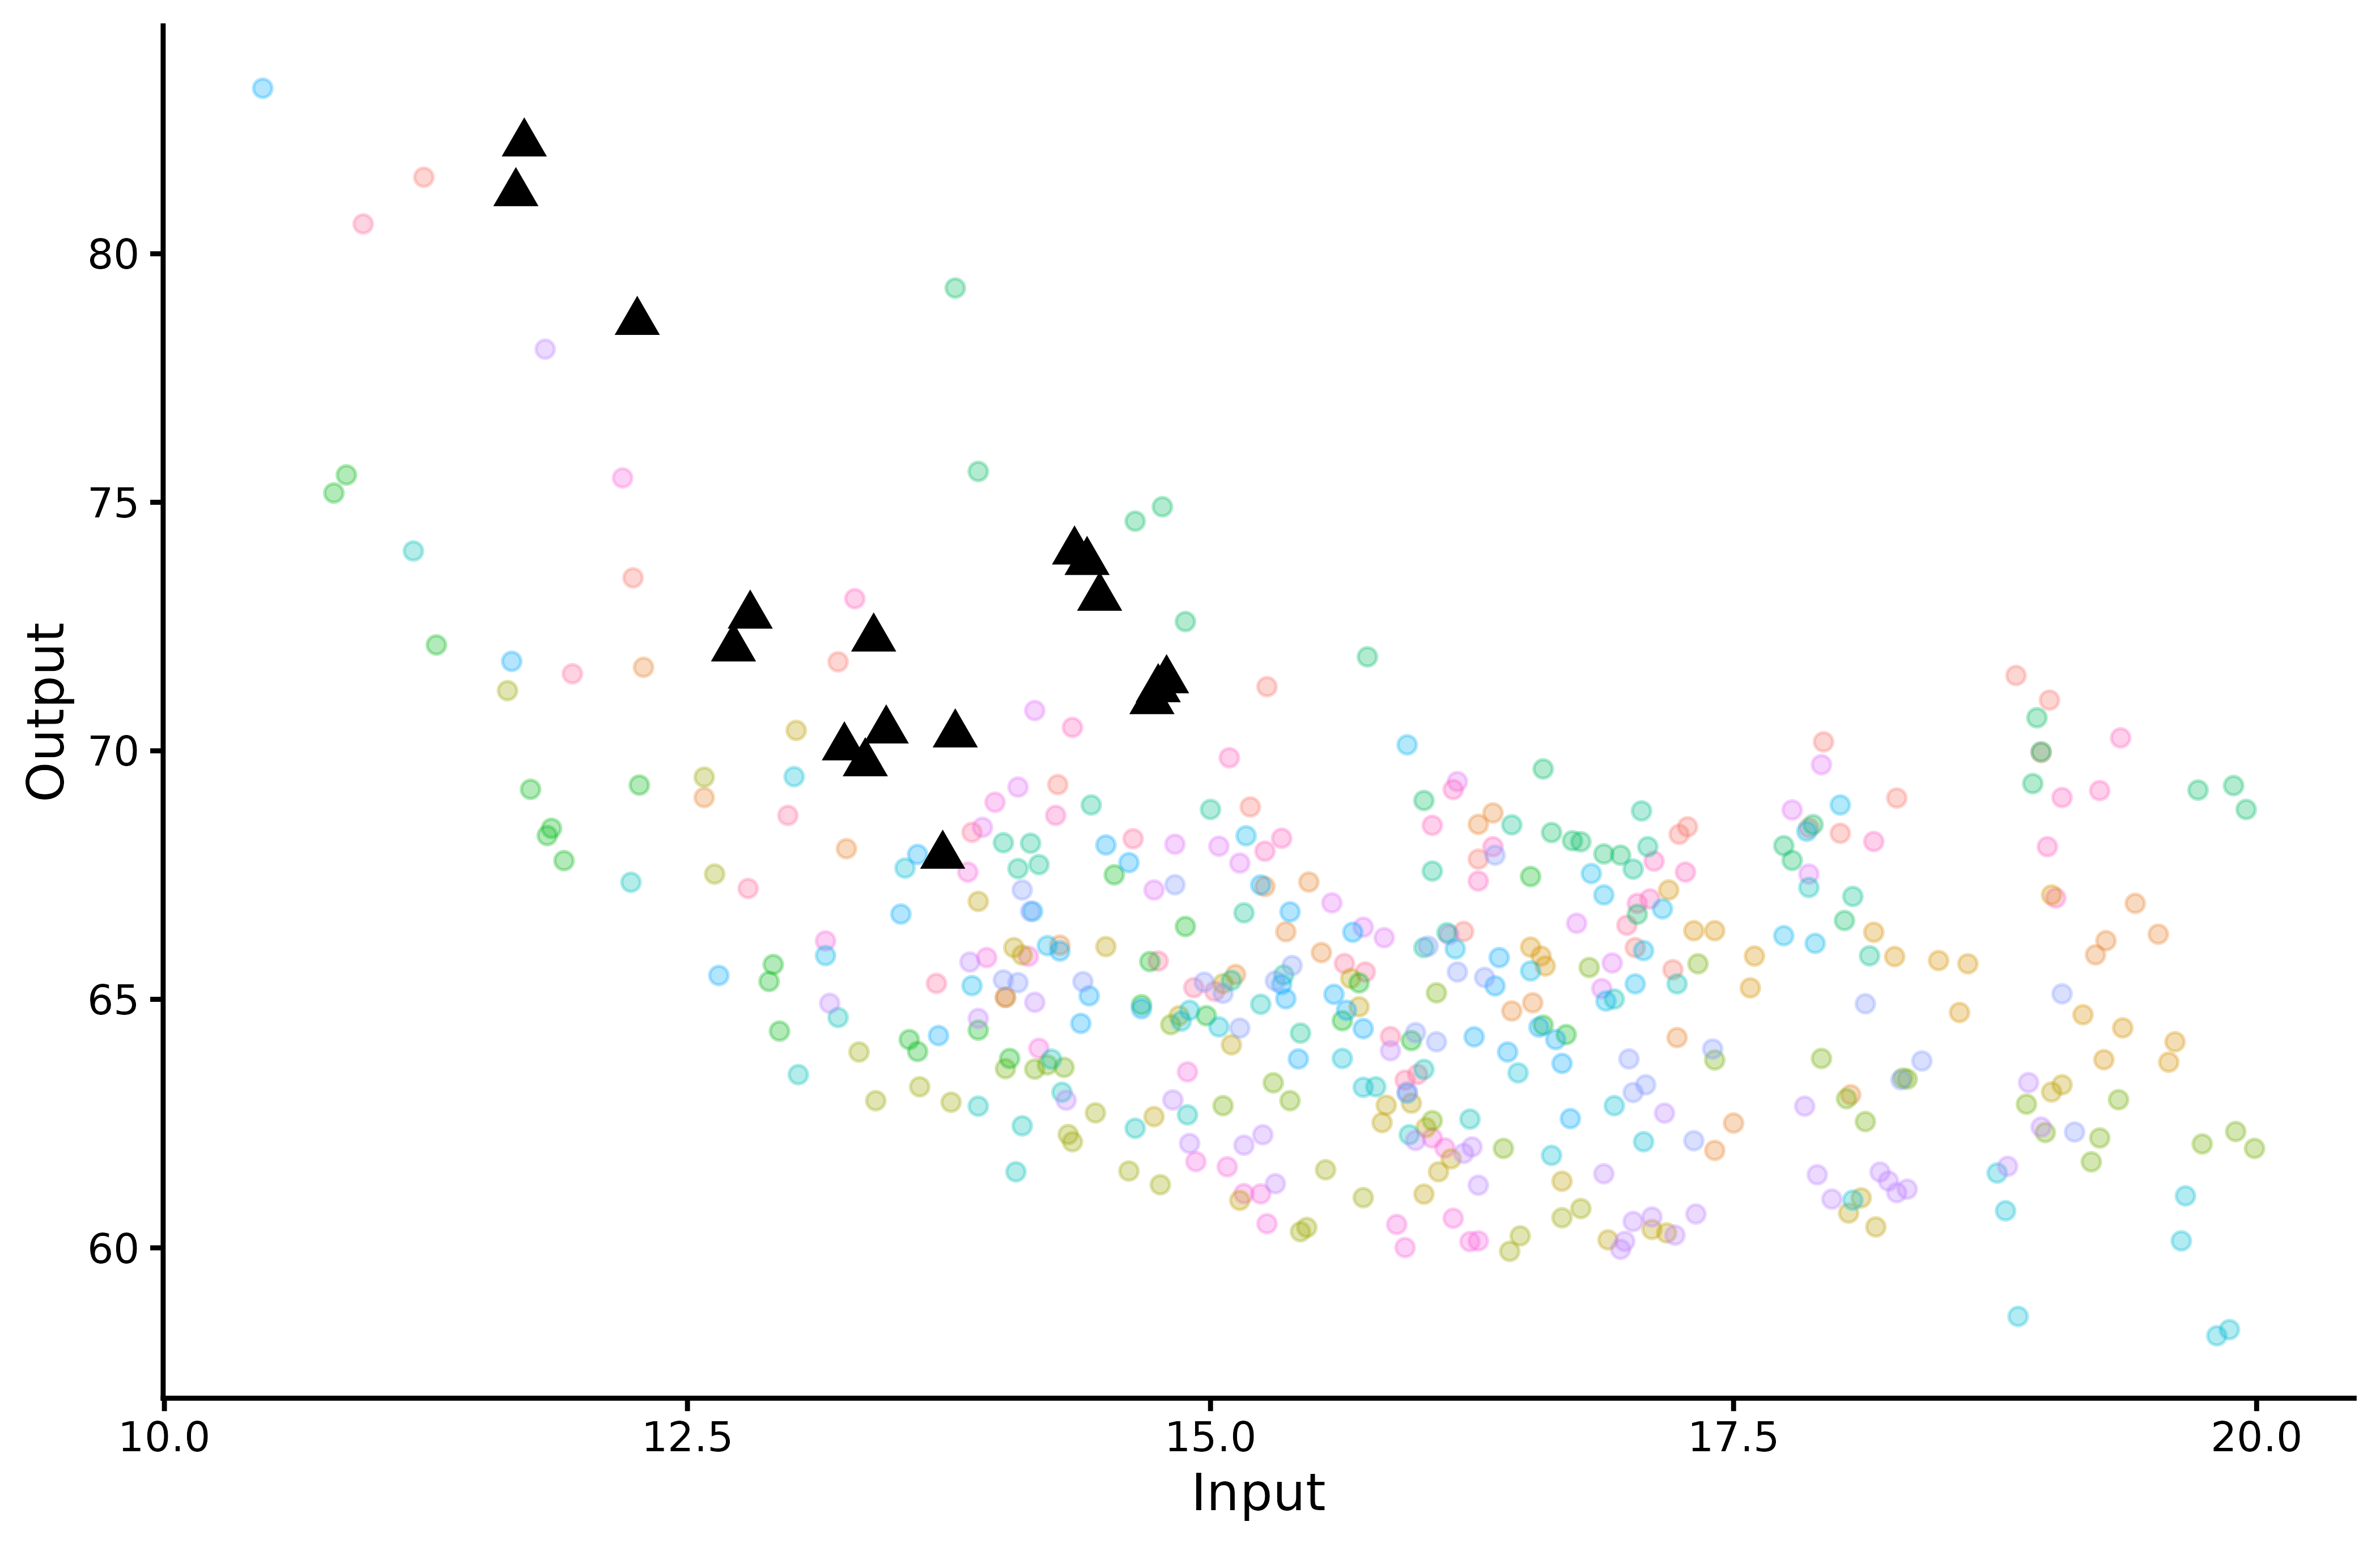
\includegraphics{Script-Package_files/figure-latex/unnamed-chunk-7-1.pdf}

\begin{verbatim}
## # A tibble: 101 x 3
##      Mean   Var Input
##     <dbl> <dbl> <dbl>
##  1 -0.751  46.8   0  
##  2 -0.829  46.6   0.1
##  3 -0.924  46.3   0.2
##  4 -1.04   45.8   0.3
##  5 -1.18   45.1   0.4
##  6 -1.35   44.0   0.5
##  7 -1.55   42.5   0.6
##  8 -1.78   40.2   0.7
##  9 -2.05   37.1   0.8
## 10 -2.35   33.0   0.9
## # ... with 91 more rows
\end{verbatim}

\hypertarget{plot-of-the-prediction-gp}{%
\subsubsection{5. Plot of the prediction /
GP}\label{plot-of-the-prediction-gp}}

\end{document}
